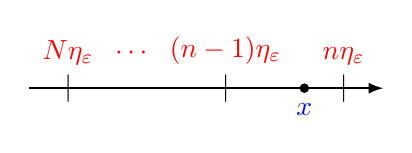
\begin{tikzpicture}[scale=5]
    \draw[-latex] [thick](-0.1,0) -- (0.8,0);
    
    \draw (0,0) node [above=5pt, red,fill=white]{$N \eta_\varepsilon$};
    \draw (0,0) node {$|$};
    
    \draw (0.16,0) node [above=7pt, red,fill=white]{$\cdots$};

    \draw (0.4,0) node [above=5pt, red,fill=white]{$(n-1) \eta_\varepsilon$};
    \draw (0.4,0) node {$|$};
    
    \draw [fill] (0.6,0) circle [radius=0.3pt];
    \draw (0.6,0) node [below=2pt, blue,fill=white]{$x$};

    \draw (0.7,0) node [above=5pt, red,fill=white]{$n \eta_\varepsilon$};
    \draw (0.7,0) node {$|$};
\end{tikzpicture}